\let\negmedspace\undefined
\let\negthickspace\undefined
\documentclass[journal]{IEEEtran}
\usepackage[a5paper, margin=10mm, onecolumn]{geometry}
\usepackage{lmodern} % Ensure lmodern is loaded for pdflatex
\usepackage{tfrupee} % Include tfrupee package

\setlength{\headheight}{1cm} % Set the height of the header box
\setlength{\headsep}{0mm}  % Set the distance between the header box and the top of the text
\usepackage{romannum}
\usepackage{csquotes}
\usepackage{gvv-book}
\usepackage{gvv}
\usepackage{circuitikz}
\usepackage{cite}
\usepackage{float}
\usepackage{amsmath,amssymb,amsfonts,amsthm}
\usepackage{algorithmic}
\usepackage{graphicx}
\usepackage{textcomp}
\usepackage{xcolor}
\usepackage{txfonts}
\usepackage{listings}
\usepackage{enumitem}
\usepackage{mathtools}
\usepackage{gensymb}
\usepackage{comment}
\usepackage[breaklinks=true]{hyperref}
\usepackage{tkz-euclide} 
\usepackage{listings}
% \usepackage{gvv}                                        
\def\inputGnumericTable{}                                 
\usepackage[latin1]{inputenc}                                
\usepackage{color}                                            
\usepackage{array}                                            
\usepackage{longtable}                                       
\usepackage{calc}                                             
\usepackage{multirow} 
\usepackage{multicol}
\usepackage{hhline}   
\usepackage{enumitem}
\usepackage{ifthen}                                           
\usepackage{lscape}
\usepackage{caption}
\usepackage{tikz}
\usetikzlibrary{patterns}

\title{GATE 2013 Question Paper (Life Sciences - XL)}
\author{EE25BTECH11019 \\ Vivek Darji}
\date{}

\begin{document}

\maketitle

\section*{General Aptitude (GA)}
\section*{Q. 1 - Q. 5 carry one mark each.} 
\begin{enumerate}
   
\item If $3 \leq X \leq 5$ and $8 \leq Y \leq 11$ then which of the following options is TRUE? \hfill $\brak{\text{GATE XL 2013}}$
\begin{enumerate}
    \item $X + Y \leq 13$
    \item $X - Y \leq -3$
    \item $X \cdot Y \leq 55$
    \item $X + Y \leq 16$
\end{enumerate}

\item  The Headmaster \underline{\rule{2cm}{0pt}} to speak to you.\\
Which of the following options is incorrect to complete the sentence? \hfill $\brak{\text{GATE XL 2013}}$
\begin{enumerate}
\begin{multicols}{4}
    \item is wanting
    \item wants
    \item want
    \item was wanting
    \end{multicols}
\end{enumerate}

\item
Mahatma Gandhi was known for his humility as \hfill $\brak{\text{GATE XL 2013}}$
\begin{enumerate}
    \item he played an important role in humiliating exit of British from India.
    \item he worked for humanitarian causes.
    \item he displayed modesty in his interactions.
    \item he was a fine human being.
\end{enumerate}

\item 
All engineering students should learn mechanics, mathematics and how to do computation.\\
Which of the underlined parts is not appropriate? \hfill $\brak{\text{GATE XL 2013}}$
\begin{enumerate}
\begin{multicols}{4}
    \item $\Romannum{1}$
    \item $\Romannum{2}$
    \item $\Romannum{3}$
    \item $\Romannum{4}$
\end{multicols}
\end{enumerate}


\item
Select the pair that best expresses a relationship similar to that expressed in the pair: \\
\textbf{water : pipe ::} \hfill $\brak{\text{GATE XL 2013}}$
\begin{enumerate}
\begin{multicols}{4}
    \item cart : road
    \item electricity : wire
    \item sea : beach
    \item music : instrument
\end{multicols}
\end{enumerate}

\section*{Q. 6 - Q. 10 carry two marks each.}

\item  
Velocity of an object fired directly in upward direction is given by $V = 80 - 32t$, where $t$ \brak{time} is in seconds. When will the velocity be between $32\,\mathrm{m/s}$ and $64\,\mathrm{m/s}$? \hfill $\brak{\text{GATE XL 2013}}$
\begin{enumerate}
\begin{multicols}{4}
    \item $\brak{1, \frac{3}{2}}$
    \item $\brak{\frac{1}{2}, 1}$
    \item $\brak{\frac{1}{2}, \frac{3}{2}}$
    \item $\brak{1, 3}$
    \end{multicols}
\end{enumerate}

\item  
In a factory, two machines $M_1$ and $M_2$ manufacture $60\%$ and $40\%$ of the auto components respectively. Out of the total production, $2\%$ of $M_1$ and $3\%$ of $M_2$ are found to be defective. If a randomly drawn auto component from the combined lot is found defective, what is the probability that it was manufactured by $M_2$? \hfill \textit\textit{\brak{GATE XL 2013}}
\begin{enumerate}
\begin{multicols}{4}
    \item 0.35
    \item 0.45
    \item 0.5
    \item 0.4
\end{multicols}
\end{enumerate}

\item  
Following table gives data on tourists from different countries visiting India in the year 2011: \hfill $\brak{\text{GATE XL 2013}}$
\begin{center}
\begin{tabular}{|l|r|}

\textbf{Country} & \textbf{Number of Tourists} \\

USA & 2000 \\
England & 3500 \\
Germany & 1200 \\
Italy & 1100 \\
Japan & 2400 \\
Australia & 2300 \\
France & 1000 \\

\end{tabular}
\end{center}
Which two countries contributed to one third of the total number of tourists who visited India in 2011?
\begin{enumerate}
    \item USA and Japan
    \item USA and Australia
    \item England and France
    \item Japan and Australia
\end{enumerate}

\item  
If $\abs{-2X + 9} = 3$ then the possible value of $\abs{-X} - X$ would be: \hfill $\brak{\text{GATE XL 2013}}$
\begin{enumerate}
\begin{multicols}{4}
    \item 30
    \item -30
    \item -42
    \item 42
\end{multicols}
\end{enumerate}

\item  
All professors are researchers.\\
Some scientists are professors.\\
Which of the given conclusions is logically valid and is inferred from the above arguments? \hfill $\brak{\text{GATE XL 2013}}$
\begin{enumerate}
    \item All scientists are researchers
    \item All professors are scientists
    \item Some researchers are scientists
    \item No conclusion follows
\end{enumerate}

\clearpage\section*{Section H: Chemistry}
\setcounter{enumi}{0}
\section*{Q. 1 - Q. 5 carry one mark each.}

\item N(CH$_3$)$_3$ and N(SiH$_3$)$_3$ are congeners, but around N-atom the former has pyramidal geometry whereas the latter is nearly planar. The bonding responsible for planarity of N(SiH$_3$)$_3$ is\hfill $\brak{\text{GATE XL 2013}}$
\begin{enumerate}
\begin{multicols}{4}
    \item p$\pi$-p$\pi$
    \item p$\pi$-d$\pi$
    \item d$\pi$-d$\pi$
    \item $\delta$
\end{multicols}
\end{enumerate}

\item The type of electronic transition responsible for the yellow colour of K$_2$CrO$_4$ is\hfill $\brak{\text{GATE XL 2013}}$
\begin{enumerate}
    \item metal to ligand charge transfer
    \item ligand to metal charge transfer
    \item intra-ligand charge transfer
    \item d-d transition
\end{enumerate}

\item The given equation $\frac{d\brak{\Delta H}}{dT} = \Delta C_p$ where $H$, $T$, and $C_p$ are the enthalpy, temperature and heat capacity at constant pressure, respectively, is called\hfill $\brak{\text{GATE XL 2013}}$
\begin{enumerate}
    \item Clausius-Clapeyron equation
    \item Hess's law
    \item Kirchhoff's equation
    \item Trouton's rule
\end{enumerate}

\section*{Q. 4 - Q. 5 are questions with numerical answer}

\item The number of 2-center-2-electron bonds in anhydrous AlCl$_3$ is \underline{\rule{2cm}{0pt}}\hfill $\brak{\text{GATE XL 2013}}$

\item When dissolved in water, the number of H$^+$ ions released from a molecule of H$_3$BO$_3$ is \underline{\rule{2cm}{0pt}}\hfill $\brak{\text{GATE XL 2013}}$

\section*{Q. 6 - Q. 15 carry two marks each.}

\item In NaCl crystal, the arrangement and coordination number of the ions are\hfill $\brak{\text{GATE XL 2013}}$
\begin{enumerate}
\begin{multicols}{4}
    \item fcc and 6
    \item fcc and 4
    \item hcp and 6
    \item hcp and 4
\end{multicols}
\end{enumerate}

\item The solubility product (K$_{sp}$) of Ca$_3$(PO$_4$)$_2$ is $1.3 \times 10^{-32}$. In a $0.02$ M solution of Ca(NO$_3$)$_2$, the solubility of Ca$_3$(PO$_4$)$_2$ (in units of M) is\hfill $\brak{\text{GATE XL 2013}}$
\begin{enumerate}
\begin{multicols}{4}
    \item $6.5 \times 10^{-9}$
    \item $1.6 \times 10^{-9}$
    \item $8.0 \times 10^{-9}$
    \item $4.0 \times 10^{-9}$
\end{multicols}
\end{enumerate}

\item Identify the \textbf{CORRECT} product in the following reaction:\hfill $\brak{\text{GATE XL 2013}}$
\begin{figure}[H]
    \centering
    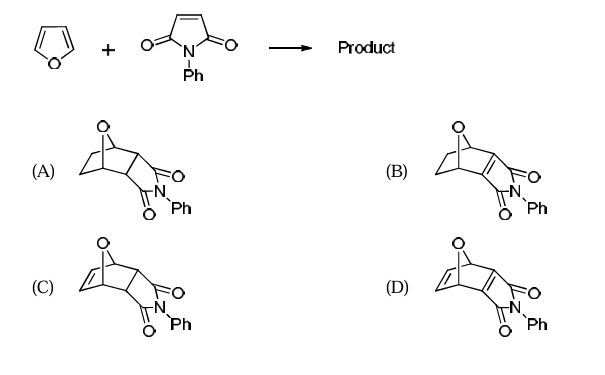
\includegraphics[width=0.9\columnwidth]{figs/xl_2013 que8 ch.png}
    \caption{Que. 8}
    \label{fig:placeholder}
\end{figure}

\item The major product obtained in the following reaction is:\hfill $\brak{\text{GATE XL 2013}}$
\begin{figure}[H]
    \centering
    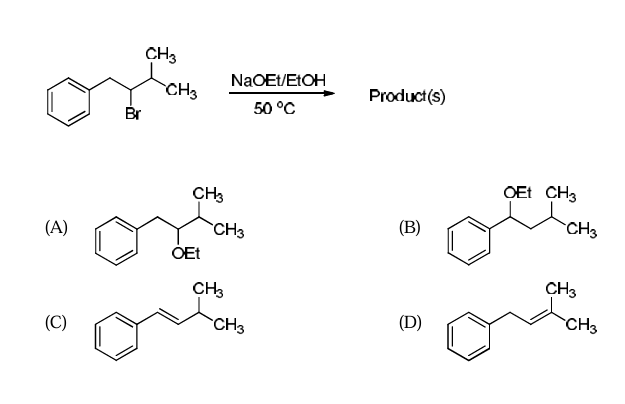
\includegraphics[width=0.9\columnwidth]{figs/xl 2013 que 9 ch.png}
    \caption{Que. 9}
    \label{fig:placeholder}
\end{figure}

\section*{Q. 10 - Q. 11 are questions with numerical answer.}

\item Iodine forms an anionic species Q in aqueous solution of iodide (I$^-$). The number of lone pair(s) of electrons on the central atom of Q is \underline{\rule{2cm}{0pt}}
\hfill $\brak{\text{GATE XL 2013}}$

\item The rate of a chemical reaction is tripled when the temperature of the reaction is increased from $298$ K to $308$ K. The activation energy (in kcal mol$^{-1}$, up to one decimal place) for the reaction is (Given $R = 1.987$ cal mol$^{-1}$ K$^{-1}$): \underline{\rule{2cm}{0pt}}\hfill $\brak{\text{GATE XL 2013}}$

\section*{Common Data for Questions 12 and 13:}

Consider the following S$_\text{N}2$ reaction of optically pure 1-chloro-3-ethylcyclopentane (\textbf{X}).
\begin{figure}[H]
    \centering
    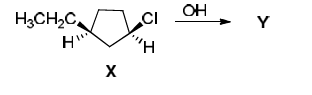
\includegraphics[width=0.85\columnwidth]{figs/Screenshot 2025-08-05 114836.png}
    \caption{common data}
\end{figure}

\item The structure of \textbf{Y} in the above reaction is\hfill $\brak{\text{GATE XL 2013}}$
\begin{figure}[H]
    \centering
    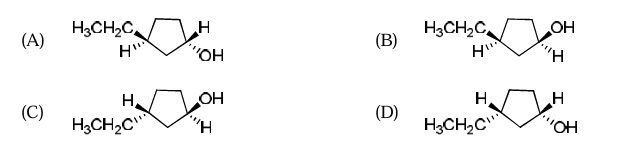
\includegraphics[width=0.85\columnwidth]{figs/Screenshot 2025-08-05 115721.png}
    \caption{12,options}
\end{figure}

\item The absolute configuration of 1-chloro-3-ethylcyclopentane shown above is\hfill $\brak{\text{GATE XL 2013}}$
\begin{enumerate}
\begin{multicols}{4}
    \item (1S,3R)
    \item (1S,3S)
    \item (1R,3R)
    \item (1R,3S)
\end{multicols}
\end{enumerate}

\section*{Linked Answer Questions}
\section*{Statement for Linked Answer Questions 14 and 15: }

\noindent\textit{The molar conductance at infinite dilution of sodium acetate, sodium sulfate and sulfuric acid solutions are $91.0 \times 10^{-4}$, $259.8 \times 10^{-4}$ and $859.3 \times 10^{-4}$ S m$^2$ mol$^{-1}$, respectively.}

\item The molar conductance at infinite dilution (in S m$^2$ mol$^{-1}$) of acetic acid is\hfill $\brak{\text{GATE XL 2013}}$
\begin{enumerate}
\begin{multicols}{4}
    \item $1028 \times 10^{-4}$
    \item $820.4 \times 10^{-4}$
    \item $690.5 \times 10^{-4}$
    \item $390.8 \times 10^{-4}$
\end{multicols}
\end{enumerate}

\item If the molar conductance of an acetic acid solution is $15.2 \times 10^{-4}$ S m$^2$ mol$^{-1}$, then the percentage dissociation of acetic acid in the solution will be:\hfill $\brak{\text{GATE XL 2013}}$
\begin{enumerate}
\begin{multicols}{4}
    \item 3.89
    \item 2.20
    \item 1.85
    \item 1.48
\end{multicols}
\end{enumerate}

\clearpage
\section*{Section I: Biochemistry}
\setcounter{enumi}{0}
\section*{Q. 1 - Q. 10 carry one mark each.}
\item Which one of the following statements is \textbf{TRUE} when a cell is kept in a hypotonic solution?\hfill $\brak{\text{GATE XL 2013}}$
\begin{enumerate}
    \item Water moves out of the cell
    \item Size of the cell remains same
    \item No movement of water takes place
    \item Size of the cell increases
\end{enumerate}

\item Which one of the following amino acids has a higher propensity for cis peptide bond formation?\hfill $\brak{\text{GATE XL 2013}}$
\begin{enumerate}
\begin{multicols}{4}
    \item Histidine
    \item Cysteine
    \item Glycine
    \item Proline
\end{multicols}
\end{enumerate}

\item The length of an $\alpha$-helix composed of 36 amino acid residues is\hfill $\brak{\text{GATE XL 2013}}$
\begin{enumerate}
\begin{multicols}{4}
    \item 10 \AA
    \item 54 \AA
    \item 27 \AA
    \item 360 \AA
\end{multicols}
\end{enumerate}

\item The order $n$ for a given substrate concentration in an enzyme catalyzed reaction following Michaelis-Menten kinetics, is\hfill $\brak{\text{GATE XL 2013}}$
\begin{enumerate}
\begin{multicols}{4}
    \item $n = 1$
    \item $n = 0$
    \item $n$ is not defined
    \item $0 \leq n \leq 1$
\end{multicols}
\end{enumerate}

\item Which one of the following amino acid residues is specifically recognised by chymotrypsin during peptide bond cleavage?\hfill $\brak{\text{GATE XL 2013}}$
\begin{enumerate}
\begin{multicols}{4}
    \item Phe
    \item Leu
    \item Val
    \item Asp
\end{multicols}
\end{enumerate}

\item The terminal electron acceptor during mitochondrial respiration is\hfill $\brak{\text{GATE XL 2013}}$
\begin{enumerate}
\begin{multicols}{4}
    \item O$_2$
    \item FAD$^+$
    \item NAD$^+$
    \item ATP
\end{multicols}
\end{enumerate}

\item During the biosynthesis of urea in the urea cycle, the two nitrogen atoms are derived from\hfill $\brak{\text{GATE XL 2013}}$
\begin{enumerate}
    \item Two free ammonium groups
    \item Free ammonium group and aspartate
    \item Both nitrogen atoms are derived from arginine
    \item One nitrogen atom from citrulline and one from glutamate
\end{enumerate}

\item An enzyme has two binding sites for an inhibitor molecule. When the inhibitor binds to the first site, the dissociation constant of the inhibitor for the second site increases, leading to negative co-operativity. The Hill coefficient for such an inhibitor is\hfill $\brak{\text{GATE XL 2013}}$
\begin{enumerate}
\begin{multicols}{4}
    \item equal to one
    \item greater than one
    \item less than one
    \item less than zero
\end{multicols}
\end{enumerate}

\item An oligonucleotide was sequenced by the dideoxy method of Sanger and the following autoradiogram was obtained:\hfill $\brak{\text{GATE XL 2013}}$
\begin{figure}[H]
    \centering
    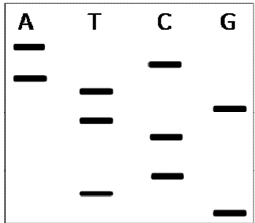
\includegraphics[width=0.75\columnwidth]{figs/Screenshot 2025-08-05 122205.png}
    \caption{que.9}
\end{figure}
The sequence of the oligonucleotide is:
\begin{enumerate}
    \item 3'-GTCCTGTACA-5'
    \item 5'-GTCCTGTACA-3'
    \item 5'-ACATGTCCTG-3'
    \item 3'-AATTTCCCGG-5'
\end{enumerate}

\item In different types of tissue transplantations, the rate of graft rejection in decreasing order is\hfill $\brak{\text{GATE XL 2013}}$
\begin{enumerate}
    \item Isograft $>$ Xenograft $>$ Allograft
    \item Allograft $>$ Isograft $>$ Xenograft
    \item Xenograft $>$ Autograft $>$ Allograft
    \item Xenograft $>$ Allograft $>$ Isograft
\end{enumerate}

\section*{Q. 11 - Q. 20 carry two marks each.}

\item You have prepared 1.0 liter of 0.5 M acetate buffer (pH = 5.0). The dissociation constant of acetic acid is $1.7 \times 10^{-5}$ M. What would be the acetate ion concentration in the buffer?\hfill  \textit{\brak{GATE XL 2013}}
\begin{enumerate}
\begin{multicols}{4}
    \item 0.1 M
    \item 0.25 M
    \item 0.315 M
    \item 0.415 M
\end{multicols}
\end{enumerate}

\item The following figures show the plot of reaction rate versus substrate concentration (mM) for an enzyme-catalyzed reaction in the presence and absence of an inhibitor. Match the possible reaction types with the plots.\hfill  \textit{\brak{GATE XL 2013}}
\begin{figure}
    \centering
    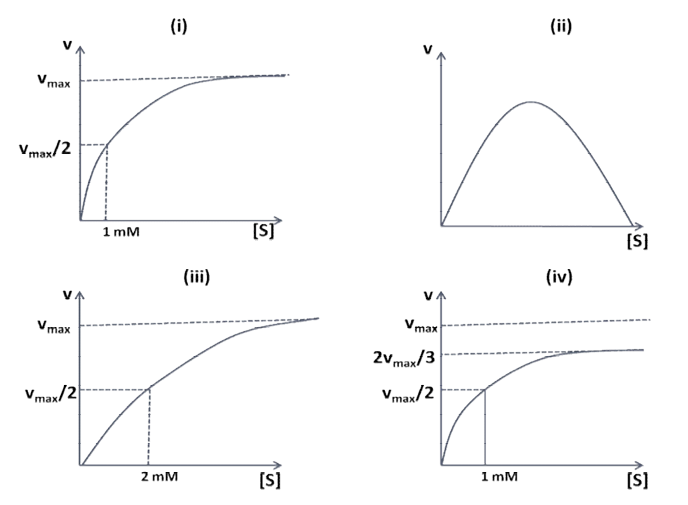
\includegraphics[width=0.5\columnwidth]{figs/Screenshot 2025-08-05 123225.png}
    \caption{que.11}
\end{figure}
\begin{enumerate}
    \item P-i, Q-iii, R-ii, S-iv
    \item P-iii, Q-ii, R-i, S-iv
    \item P-iii, Q-iv, R-i, S-ii
    \item P-iv, Q-ii, R-i, S-iii
\end{enumerate}

\item Arrange the following in the decreasing order of their permeability coefficients across a lipid bilayer membrane.\hfill $\brak{\text{GATE XL 2013}}$
\begin{enumerate}
    \item (i), (iii), (v), (ii), (iv)
    \item (iii), (v), (ii), (iv), (i)
    \item (iii), (i), (v), (ii), (iv)
    \item (i), (iii), (iv), (v), (ii)
\end{enumerate}

\item Arrange the following in the increasing order of amount of ATP generated by metabolism of one molecule of the following compounds:\hfill  \textit{\brak{GATE XL 2013}}
\begin{enumerate}
    \item (ii), (iv), (iii), (i)
    \item (iii), (ii), (i), (iv)
    \item (iv), (ii), (i), (iii)
    \item (iii), (ii), (iv), (i)
\end{enumerate}

\item Match the following enzymes with their regulatory mechanisms:\hfill  \textit{\brak{GATE XL 2013}}
\begin{enumerate}
    \item (a)-3, (b)-2, (c)-1, (d)-4
    \item (a)-3, (b)-4, (c)-2, (d)-1
    \item (a)-4, (b)-3, (c)-1, (d)-4
    \item (a)-4, (b)-1, (c)-2, (d)-3
\end{enumerate}

\item A researcher wants to clone 3 DNA fragments of sizes 1.1 Mb, 0.097 Mb and 0.045 Mb. The choice of the vectors for cloning each of the fragments are\hfill  \textit{\brak{GATE XL 2013}}
\begin{enumerate}
    \item Cosmid, bacteriophage $\lambda$, bacteriophage P1
    \item Yeast artificial chromosome, bacteriophage P1, cosmid
    \item Bacterial artificial chromosome, bacteriophage $\lambda$, yeast artificial chromosome
    \item Only plasmids
\end{enumerate}

\item Which of the four restriction enzymes given below cut the following DNA sequence?\\
5'-CCGATATCTCGAGGGC-3'\hfill  \textit{\brak{GATE XL 2013}}
\begin{enumerate}
\begin{multicols}{4}
    \item P \& Q
    \item P, R \& S
    \item Q \& S
    \item P \& R
\end{multicols}
\end{enumerate}

\item You have expressed the following protein that has an isoelectric point of 6.0. The best order of protein purification methodologies to obtain a pure protein is?\hfill  \textit{\brak{GATE XL 2013}}
\begin{figure}
    \centering
    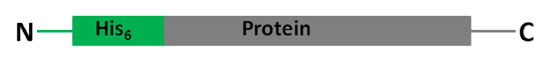
\includegraphics[width=0.5\columnwidth]{figs/Screenshot 2025-08-05 123543.png}
    \caption{Que. 18}
\end{figure}
\begin{enumerate}
    \item Gel filtration chromatography, Anion exchange chromatography at pH = 4.0, Ammonium sulphate precipitation
    \item Cation exchange chromatography at pH = 9.0, Ni-affinity chromatography, Gel filtration chromatography
    \item Anion exchange chromatography at pH = 8.0, Ni-affinity chromatography, Gel filtration chromatography
    \item Ammonium sulphate precipitation, Anion exchange chromatography at pH = 4.0, Ni-affinity chromatography
\end{enumerate}

\item An enzyme of 40 kDa is added to a substrate solution in a molar ratio of 1:3. The concentration of the enzyme in the mixture is 12 mg/ml. What would be the corresponding substrate concentration?\hfill  \textit{\brak{GATE XL 2013}}
\begin{enumerate}
\begin{multicols}{4}
    \item 0.4 mM
    \item 0.12 mM
    \item 0.9 mM
    \item 0.3 mM
\end{multicols}
\end{enumerate}

\item A patient suffering from pneumonia and tuberculosis was found to have very low CD4$^+$ T cells. In all probability the \textbf{PRIMARY} causative infectious agent belongs to\hfill  \textit{\brak{GATE XL 2013}}
\begin{enumerate}
    \item Klebsiella family
    \item Mycobacterium family
    \item Retrovirus family
    \item Streptococcus family
\end{enumerate}

\clearpage
\section*{Section J: Botany}
\setcounter{enumi}{0}
\section*{Q. 1 - Q. 10 carry one mark each.}

\item Bast fibres are present in\hfill  \textit{\brak{GATE XL 2013}}
\begin{enumerate}
\begin{multicols}{4}
    \item Xylem
    \item Phloem
    \item Collenchyma
    \item Parenchyma
\end{multicols}
\end{enumerate}

\item During cellular respiratory process, pyruvate must be oxidized to acetyl CoA and CO$_2$ before it enters the citric acid cycle. The simplified equation is: \\
\texttt{Pyruvate + NAD$^+$ + CoASH $\rightarrow$ Acetyl-S-CoA + NADH + CO$_2$} \\
This oxidation occurs in mitochondria and is carried out by the enzyme:\hfill  \textit{\brak{GATE\ }}
\begin{enumerate}
    \item Pyruvate kinase
    \item Pyruvate dehydrogenase
    \item Pyruvate decarboxylase
    \item Pyruvate carboxylase
\end{enumerate}

\item Which of the following statements is \textbf{CORRECT}?\hfill  \textit{\brak{GATE XL 2013}}
\begin{enumerate}
    \item The rice gene contains about 50,000 genomes on 12 chromosomes
    \item The rice genome contains about 50,000 genes on 12 chromosomes
    \item The rice chromosome contains about 50,000 genes on 12 genomes
    \item The rice genome contains about 50,000 chromosomes on 12 genes
\end{enumerate}

\item The aflatoxin found in post-harvested grains is injurious due to\hfill  \textit{\brak{GATE XL 2013}}
\begin{enumerate}
\begin{multicols}{4}
    \item Aspergillus
    \item Alternaria
    \item Fusarium
    \item Phytopthora
\end{multicols}
\end{enumerate}

\item Identify the event that exclusively occurs in meiotic cell division:\hfill  \textit{\brak{GATE XL 2013}}
\begin{enumerate}
\begin{multicols}{4}
    \item Chromatid formation
    \item Spindle formation
    \item Synapsis
    \item Chromosome movement to pole
\end{multicols}
\end{enumerate}

\item In nitrogen fixation, leghemoglobin helps in the presence of\hfill  \textit{\brak{GATE XL 2013}}
\begin{enumerate}
\begin{multicols}{4}
    \item Nitrate synthetase
    \item Nitrate synthase
    \item Glutathione synthetase
    \item Nitrogenase
\end{multicols}
\end{enumerate}

\item Identify the \textbf{INCORRECT} statement:\hfill  \textit{\brak{GATE XL 2013}}
\begin{enumerate}
    \item Detrital food chain energy flow is hard to measure
    \item Ecological succession is change in community over time
    \item Pollution reflects solar energy back, slowing warming
    \item Photoperiodism has no relation to ecosystem
\end{enumerate}

\item Two enzymes commonly used for plant protoplast isolation are\hfill  \textit{\brak{GATE XL 2013}}
\begin{enumerate}
    \item Cellulase and Lipase
    \item Cellulase and Amylase
    \item Pectinase and Cellulase
    \item Pectinase and Lipase
\end{enumerate}

\item For successful transfer of a gene using Ti-plasmid, essential components are\hfill  \textit{\brak{GATE XL 2013}}
\begin{enumerate}
    \item Opine catabolism genes, Left border, Right border
    \item Opine catabolism genes, Left border, Virulence genes
    \item Hormone genes, Right border, Virulence genes
    \item Left border, Right border, Virulence genes
\end{enumerate}

\item In cytoplasmic male sterility, the determinant is located in\hfill  \textit{\brak{GATE XL 2013}}
\begin{enumerate}
\begin{multicols}{4}
    \item Chloroplast
    \item ER
    \item Golgi
    \item Mitochondria
\end{multicols}
\end{enumerate}

\section*{Q. 11 - Q. 20 carry two marks each.}

\item Match the floral formula with family and species:\hfill  \textit{\brak{GATE XL 2013}}
\begin{enumerate}
    \item P-1-iv, Q-2-iii, R-6-i, S-4-ii
    \item P-2-v, Q-4-vi, R-3-iii, S-5-iv
    \item P-3-v, Q-6-iii, R-5-i, S-2-ii
    \item P-3-vi, Q-4-i, R-1-v, S-5-ii
\end{enumerate}

\item A plant of genotype GGHH is crossed with gghh. If F1 is test-crossed, what percentage of progeny will be gghh in these cases?\hfill  \textit{\brak{GATE XL 2013}}
\begin{enumerate}
    \item P-25, Q-25, R-25, S-25
    \item P-25, Q-50, R-45, S-38
    \item P-50, Q-50, R-90, S-76
    \item P-25, Q-50, R-10, S-24
\end{enumerate}

\item Which two statements are \textbf{CORRECT}?\hfill  \textit{\brak{GATE XL 2013}}
\begin{enumerate}
\begin{multicols}{4}
    \item P,Q
    \item Q,R
    \item R,S
    \item P,S
\end{multicols}
\end{enumerate}

\item Match the natural products:\hfill  \textit{\brak{GATE XL 2013}}
\begin{enumerate}
    \item P-3-iv, Q-4-ii, R-2-v, S-6-i
    \item P-2-iii, Q-3-i, R-1-iv, S-5-v
    \item P-3-iv, Q-4-ii, R-2-v, S-6-i
    \item P-4-iii, Q-1-v, R-5-i, S-2-vi
\end{enumerate}

\item Which two statements are \textbf{INCORRECT}?\hfill  \textit{\brak{GATE XL 2013}}
\begin{enumerate}
\begin{multicols}{4}
    \item P,Q
    \item Q,R
    \item Q,S
    \item P,R
\end{multicols}
\end{enumerate}

\item Which of the following are synthetic analogues of auxin and cytokinin?\hfill  \textit{\brak{GATE XL 2013}}
\begin{enumerate}
    \item IAA and Kinetin
    \item 2,4-D and Zeatin
    \item IAA and Zeatin
    \item 2,4-D and Kinetin
\end{enumerate}

\item Which two statements are \textbf{INCORRECT}?\hfill  \textit{\brak{GATE XL 2013}}
\begin{enumerate}
\begin{multicols}{4}
    \item P,R
    \item Q,S
    \item Q,R
    \item P,S
\end{multicols}
\end{enumerate}

\item Identify two \textbf{CORRECT} traits for:\hfill  \textit{\brak{GATE XL 2013}}
\begin{enumerate}
    \item P-1,3; Q-2,4
    \item P-2,4; Q-1,3
    \item P-1,4; Q-2,3
    \item P-2,3; Q-1,4
\end{enumerate}

\item Match the enzyme terms:\hfill  \textit{\brak{GATE XL 2013}}
\begin{enumerate}
    \item P-4, Q-5, R-2, S-3
    \item P-4, Q-3, R-1, S-2
    \item P-4, Q-3, R-5, S-6
    \item P-4, Q-1, R-3, S-5
\end{enumerate}

\item Choose two \textbf{CORRECT} statements on ion transport in roots:\hfill  \textit{\brak{GATE XL 2013}}
\begin{enumerate}
\begin{multicols}{4}
    \item P,S
    \item Q,R
    \item R,S
    \item Q,S
\end{multicols}
\end{enumerate}

\clearpage
\section*{Section K: Microbiology}
\setcounter{enumi}{0}
\section*{Q. 1 - Q. 10 carry one mark each.}
\begin{enumerate}[label=\arabic*.]
\item In 1976, Tonegawa's experiment gave clue about gene rearrangement during differentiation of B-cells. The two different types of cells used in this experiment were
\begin{enumerate}
\item HeLa cells and fibrosarcoma cells
\item embryonic cells and fibroblasts
\item adult myeloma cells and HeLa cells
\item embryonic cells and adult myeloma cells
\end{enumerate}
\hfill $\brak{\text{GATE XL 2013}}$

\item To which one of the following groups, the antibiotics kanamycin, streptomycin and gentamicin belong?
\begin{enumerate}
\begin{multicols}{4}
\item cephalosporins
\item macrolides
\item aminoglycosides
\item quinolones
\end{multicols}
\end{enumerate}
\hfill $\brak{\text{GATE XL 2013}}$

\item Shine Dalgarno's sequence present in mRNA binds to
\begin{enumerate}
\begin{multicols}{4}
\item 3$^{\prime}$ end of rRNA
\item 5$^{\prime}$ end of rRNA
\item 5$^{\prime}$ end of tRNA
\item 3$^{\prime}$ end of tRNA
\end{multicols}
\end{enumerate}
\hfill $\brak{\text{GATE XL 2013}}$

\item Which one of the following transport mechanisms is NOT employed by prokaryotes?
\begin{enumerate}
\begin{multicols}{4}
\item Passive diffusion
\item Group translocation
\item Endocytosis
\item Active transport
\end{multicols}
\end{enumerate}
\hfill $\brak{\text{GATE XL 2013}}$

\item The most common indicator organism of faecal pollution in water is
\begin{enumerate}
\begin{multicols}{4}
\item \textit{Clostridium botulinum}
\item \textit{Bacillus subtilis}
\item \textit{Escherichia coli}
\item \textit{Clostridium tetani}
\end{multicols}
\end{enumerate}
\hfill $\brak{\text{GATE XL 2013}}$

\item The theoretical maximum number of ATP molecules produced from aerobic oxidation of glucose by eukaryotic cells is
\begin{enumerate}
\begin{multicols}{4}
\item 38
\item 24
\item 12
\item 8
\end{multicols}
\end{enumerate}
\hfill $\brak{\text{GATE XL 2013}}$

\item Which one of the following DO NOT use water as an electron source during photosynthesis?
\begin{enumerate}
\item Sulfate reducing bacteria
\item Methanogenic bacteria
\item Green and purple bacteria
\item Nitrifying bacteria
\end{enumerate}
\hfill $\brak{\text{GATE XL 2013}}$

\item If the radius of a spherical coccus is $0.8\,\mu\text{m}$, the value of surface area to volume ratio in $\mu\text{m}^{-1}$ will be
\begin{enumerate}
\begin{multicols}{4}
\item 7.45
\item 4.05
\item 3.75
\item 0.85
\end{multicols}
\end{enumerate}
\hfill $\brak{\text{GATE XL 2013}}$

\item The enzyme that catalyzes the reduction of nitrogen to ammonia is
\begin{enumerate}
\begin{multicols}{4}
\item nitrogenase
\item nitrate reductase
\item nitrite reductase
\item deaminase
\end{multicols}
\end{enumerate}
\hfill $\brak{\text{GATE XL 2013}}$

\item Chemostat is a continuous culture system in which sterile medium is fed into the culture vessel at the same rate as the spent medium is removed. If in a chemostat culture, the flow rate is $30\,\text{ml}\,\text{h}^{-1}$ and volume of the medium inside the vessel is $100\,\text{ml}$, the dilution rate in $\text{h}^{-1}$ is
\begin{enumerate}
\begin{multicols}{4}
\item 3.33
\item 1.50
\item 0.75
\item 0.30
\end{multicols}
\end{enumerate}
\hfill $\brak{\text{GATE XL 2013}}$
\end{enumerate}

\section*{Q. 11 - Q. 20 carry two marks each.}

\begin{enumerate}[label=\arabic*., start=11]
\item In an experiment the structural genes \textit{lacZYA} of lac operon were found to be constitutively expressed. The following explanations were given:  
\brak{P} absence of a functional repressor due to mutation in the repressor gene \textit{lacI}  
\brak{Q} mutation in the operator that can no longer bind the repressor  
\brak{R} mutation in the \textit{lacA} gene  
Which of the following is CORRECT?
\begin{enumerate}
\begin{multicols}{4}
\item Only P
\item Only Q
\item Both P \& Q
\item Only R
\end{multicols}
\end{enumerate}
\hfill $\brak{\text{GATE XL 2013}}$

\item Which one of the following is TRUE about siderophores in bacteria?
\begin{enumerate}
\item Secreted only when soluble iron is available
\item Form complex with ferrous ions in medium
\item Are the only route of iron uptake
\item Form complex with ferric ions in medium
\end{enumerate}
\hfill $\brak{\text{GATE XL 2013}}$

\item In a population containing fast and slow growing bacteria, the slow growing bacteria can be enriched by supplementing the medium with
\begin{enumerate}
\item chloramphenicol
\item penicillin
\item penicillin \& chloramphenicol
\item rifampin
\end{enumerate}
\hfill $\brak{\text{GATE XL 2013}}$

\item When the supply of tryptophan is plentiful, the tryptophan operon is repressed because
\begin{enumerate}
\item repressor protein-corepressor complex is bound at operator
\item repressor protein is synthesized in large quantity
\item repressor-corepressor complex is not formed
\item repressor becomes inactive and reduces operator binding
\end{enumerate}
\hfill $\brak{\text{GATE XL 2013}}$

\item Match the scientists in Group I with their contributions in Group II:  
\begin{tabular}{ll}
\textbf{Group I} & \textbf{Group II} \\
P. Robert Hooke & I. Proved that microbes cause diseases \\
Q. Paul Ehrlich & II. First to observe cells \\
R. Antony van Leeuwenhoek & III. First to observe bacteria \\
S. Sergei Winogradsky & IV. First synthetic chemotherapeutic agent \\
& V. Linked specific bacteria to biogeochemical cycles \\
\end{tabular}
\begin{enumerate}
\item P-I, Q-II, R-III, S-V
\item P-II, Q-IV, R-III, S-V
\item P-II, Q-I, R-III, S-IV
\item P-V, Q-III, R-IV, S-II
\end{enumerate}
\hfill $\brak{\text{GATE XL 2013}}$

\item Match the infectious agents in Group I with associated diseases in Group II:  
\begin{tabular}{ll}
\textbf{Group I} & \textbf{Group II} \\
P. \textit{Bordetella pertussis} & I. Mumps \\
Q. \textit{Mycobacterium leprae} & II. Meningitis \\
R. \textit{Haemophilus influenzae} & III. Tuberculosis \\
S. Rubella & IV. Whooping cough \\
& V. Hansen's disease \\
\end{tabular}
\begin{enumerate}
\item P-IV, Q-V, R-II, S-I
\item P-V, Q-III, R-I, S-IV
\item P-I, Q-III, R-V, S-IV
\item P-III, Q-II, R-V, S-I
\end{enumerate}
\hfill $\brak{\text{GATE XL 2013}}$

\item Match the microscopes in Group I with their working principles in Group II:  
\begin{tabular}{ll}
\textbf{Group I} & \textbf{Group II} \\
P. Phase contrast & I. Light from sides only \\
Q. Dark field & II. Uses fluorescent dyes \\
R. Bright field & III. RI difference from medium \\
S. Electron microscopy & IV. Contrast difference from background \\
& V. Uses electrons instead of photons \\
\end{tabular}
\begin{enumerate}
\item P-V, Q-II, R-III, S-V
\item P-III, Q-I, R-IV, S-V
\item P-III, Q-II, R-V, S-I
\item P-II, Q-I, R-III, S-V
\end{enumerate}
\hfill $\brak{\text{GATE XL 2013}}$

\item In a phenol coefficient test for disinfectant X, effective dilution for X and phenol were $1/450$ and $1/90$. Calculate the phenol coefficient.
\begin{enumerate}
\begin{multicols}{4}
\item 10.0
\item 5.0
\item 1.0
\item 0.2
\end{multicols}
\end{enumerate}
\hfill $\brak{\text{GATE XL 2013}}$

\item How many electrons are accepted when sulfate acts as the terminal electron acceptor in \textit{Desulfovibrio}?
\begin{enumerate}
\begin{multicols}{4}
\item 8
\item 6
\item 4
\item 2
\end{multicols}
\end{enumerate}
\hfill $\brak{\text{GATE XL 2013}}$

\item A bacterial population increases from $10^3$ cells to $10^9$ cells in 10 hours. Calculate the number of generations per hour.
\begin{enumerate}
\begin{multicols}{4}
\item 20
\item 10
\item 4
\item 2
\end{multicols}
\end{enumerate}
\hfill $\brak{\text{GATE XL 2013}}$
\end{enumerate}
\clearpage
\section*{Section L: Zoology}
\setcounter{enumi}{0}
\section*{Q. 1 - Q. 10 carry one mark each.}

\item Which one of the following provides the strongest support for the theory of 'descent with modification'? \hfill $\brak{\text{GATE XL 2013}}$
\begin{enumerate}
    \item Early embryonic forms of diverse organisms (examples: fishes, birds and mammals) appear similar
    \item Ability of fishes and whales to swim
    \item Variation in flower colour in a given species
    \item Skin colour variation among individuals in a human population
\end{enumerate}

\item Which one of the following is an example of sympatric speciation? \hfill $\brak{\text{GATE XL 2013}}$
\begin{enumerate}
    \item Origin of new species among wasps that pollinate figs
    \item Emergence of a new species among finches that migrated to an island and thus isolated from their ancestors
    \item Evolution of birds' and bats' wings
    \item Speciation of squirrels separated by a wide river
\end{enumerate}

\item The primary difference between glycogen and cellulose is in the \hfill $\brak{\text{GATE XL 2013}}$
\begin{enumerate}
    \item types of constituent monosaccharides
    \item number of monomers per molecule
    \item configuration of the monomers
    \item susceptibility to acid hydrolysis
\end{enumerate}

\item Control mechanisms operate at any of the several steps involved in gene expression. Which one of the following is the key mode of regulation during the cell cycle? \hfill $\brak{\text{GATE XL 2013}}$
\begin{enumerate}
    \item Transcription
    \item mRNA processing
    \item Activation of protein function resulting from protein-protein interaction
    \item mRNA export
\end{enumerate}

\item Testicular feminization syndrome is a genetic condition wherein an individual with a XY genotype will have an external female-like phenotype. This is caused by \hfill $\brak{\text{GATE XL 2013}}$
\begin{enumerate}
    \item Functional loss of androgen receptor
    \item Increased production of estrogen and its receptor
    \item Functional loss of Mullerian inhibiting hormone
    \item Functional loss of androgen receptor and Mullerian inhibiting hormone
\end{enumerate}

\item Which one of the following defects do you expect to see if you were able to specifically block apoptosis in the developing limb bud of a frog embryo? \hfill $\brak{\text{GATE XL 2013}}$
\begin{enumerate}
    \item The digits will remain connected through a web-like extension
    \item The bones will not form, and the limb would look like a paddle
    \item The limb would look normal but would be larger in size
    \item The anterior-posterior polarity of the limb will be lost
\end{enumerate}

\item The formation of antigen-antibody complex helps in disposing antigen through the following pathways EXCEPT: \hfill $\brak{\text{GATE XL 2013}}$
\begin{enumerate}
    \item Neutralizing the antigen by blocking its activity
    \item By directly hydrolyzing the antigen
    \item By promoting the precipitation of antigen
    \item By activating cell lysis pathway
\end{enumerate}

\item The term 'ecological succession' refers to: \hfill $\brak{\text{GATE XL 2013}}$
\begin{enumerate}
    \item A process wherein newer species populate a region that was devoid of flora and fauna
    \item A transition phase wherein one particular set of species is replaced by another set of species
    \item Changes in the community due to a disturbance in the habitat
    \item All the above
\end{enumerate}

\item Which one of the following options provide example for the term 'habituation' in behavioral ecology? \hfill $\brak{\text{GATE XL 2013}}$
\begin{enumerate}
    \item A fish transferred to a fish tank startles initially for a hand clap, but not later
    \item Migratory birds from the temperate zone migrating towards the tropical part during the winters
    \item Adult kingfisher birds are more successful in catching fishes than their younger siblings
    \item Female lizard getting used to a new male lizard during the courtship period
\end{enumerate}

\item Among the following cell structure-function pairs, identify the correctly paired one \hfill $\brak{\text{GATE XL 2013}}$
\begin{enumerate}
    \item Microvilli - engulfment of foreign bodies
    \item Cytoskeleton - cell migration
    \item Peroxisomes - cellular respiration
    \item Nucleolus - mRNA transcription
\end{enumerate}

\section*{Q. 11 - Q. 20 carry two marks each.}

\item Which of the following most accurately states the goal of systematics? \hfill $\brak{\text{GATE XL 2013}}$
\begin{enumerate}
    \item Classification scheme should reflect phylogenetic relationship
    \item All animals should be classified based on the relatedness at the early embryonic stage
    \item All animals should be grouped based on DNA sequence data
    \item Classification of animals should be based on morphological characters
\end{enumerate}

\item Among the following options, choose the one that is probably a cause of rapid diversification of animal groups during the Cambrian explosion. \hfill $\brak{\text{GATE XL 2013}}$
\begin{enumerate}
    \item Adaptation of organisms to live in the salty environment of ocean
    \item Emergence of coelom
    \item The movement of animals to land
    \item The accumulation of sufficient atmospheric oxygen to support the metabolism of actively moving animals
\end{enumerate}

\item A newly discovered, recessively-inherited disease-susceptibility trait \brak{D} is observed only in cotton plants with white flowers, although the flower colour \brak{R} and DS are independently inherited. In a breeding programme, one variety that is homozygous for the absence of DS, but heterozygous for R was mated to another having white flowers but heterozygous for DS. What is the probability that a given plant among the cross progeny will be susceptible to the disease? \hfill $\brak{\text{GATE XL 2013}}$
\begin{enumerate}
\begin{multicols}{4}
    \item 25\%
    \item 12.5\%
    \item 75\%
    \item 0\%
\end{multicols}
\end{enumerate}

\item In a new species of moth, the genes for body colour \brak{B/b}, wing size \brak{W/w}, and eye colour \brak{R/r} are linked. Recombination frequencies: B-W: 5\%, R-W: 15\%, B-R: 10\%. Which among the following is the correct order of these three genetic loci? \hfill $\brak{\text{GATE XL 2013}}$
\begin{enumerate}
    \item Body colour - Eye colour - Wing size
    \item Eye colour - Wing size - Body colour
    \item Wing size - Body colour - Eye colour
    \item Eye colour - Body colour - Wing size
\end{enumerate}

\item From the options given below, identify the correct combination that truly represents the adaptation seen in desert mammals: \hfill $\brak{\text{GATE XL 2013}}$
\begin{enumerate}
    \item Options i and iii
    \item Options ii and iii
    \item Options i and iv
    \item Options i and v
\end{enumerate}

\item In \textit{Drosophila}, mutations in homeotic genes result in which one of the following developmental defects? \hfill $\brak{\text{GATE XL 2013}}$
\begin{enumerate}
    \item The anterior portion of the embryo will not develop
    \item Several segments in the anterior region of the embryo will be lost
    \item Segmentation will be lost, and the embryo will have only one segment
    \item Segment-specific identities will be lost
\end{enumerate}

\item Retroviruses escape pre-existing antibodies in the host by: \hfill $\brak{\text{GATE XL 2013}}$
\begin{enumerate}
    \item Editing the surface antigen post-translationally
    \item RNA polymerase of these viruses having high mutation rate
    \item Surface antigens are attacked by host proteases
    \item Host DNA polymerase mutates the viral genome
\end{enumerate}

\item Match the following age structure patterns with their implications: \hfill $\brak{\text{GATE XL 2013}}$
\begin{enumerate}
    \item I-ii; II-iii; III-iv; IV-i
    \item I-ii; II-iii; III-ii; IV-iv
    \item I-i; II-ii; III-iii; IV-iv
    \item I-i; II-iii; III-ii; IV-iv
\end{enumerate}

\item Which one of the following examples is NOT true with regard to the evolution of behavior by natural selection? \hfill $\brak{\text{GATE XL 2013}}$
\begin{enumerate}
    \item The behavioral trait is determined only by genes
    \item The behavioral trait varies within the population of that species
    \item The reproductive success partly depends on the behavioral trait
    \item The behavioral trait is influenced by the genotype
\end{enumerate}

\item Among the following molecular process-biological effect pairs, identify the mismatched pair. \hfill $\brak{\text{GATE XL 2013}}$
\begin{enumerate}
    \item Histone deacetylation - activation of gene expression
    \item Protein phosphorylation - signal transduction
    \item DNA methylation - sex-specific control of gene expression
    \item Proteolytic cleavage - activation of signaling by peptide hormones
\end{enumerate}

\clearpage
\section*{Section M: Food Technology}
\setcounter{enumi}{0}
\section*{Q. 1 - Q. 10 carry one mark each.}

\item Kawashiorkor disease is caused due to the deficiency of\hfill $\brak{\text{GATE XL 2013}}$
\begin{enumerate}
\item lysine
\item unsaturated fatty acids
\item vitamin K
\item protein

\end{enumerate}

\item Which of the following statements is TRUE in case of oxidative rancidity of vegetable oils and fats?\hfill $\brak{\text{GATE XL 2013}}$
\begin{enumerate}
    \item It is caused by the reaction of saturated fatty acids and oxygen
    \item It involves polymerization of fatty acids
    \item It is caused by the reaction of unsaturated fatty acids with oxygen
    \item It is caused by oxidative enzymes
\end{enumerate}

\item The food borne disease, Q fever is caused by the organism\hfill $\brak{\text{GATE XL 2013}}$
\begin{enumerate}
    \item \textit{Clostridium perfringens}
    \item \textit{Coxiella burnetii}
    \item \textit{Bacillus cereus}
    \item \textit{Staphylococcus aureus}
\end{enumerate}

\item The primary bacterial spoilage of poultry meat at low temperature, with characteristic sliminess at outer surface, is caused by\hfill $\brak{\text{GATE XL 2013}}$
\begin{enumerate}
\begin{multicols}{4}
    \item \textit{Pseudomonas spp.}
    \item \textit{Aspergillus spp.}
    \item \textit{Bacillus spp.}
    \item \textit{Candida spp.}
\end{multicols}
\end{enumerate}

\item The weight gain \brak{in\  gram} per gram protein consumed is called\hfill $\brak{\text{GATE XL 2013}}$
\begin{enumerate}
    \item Net Protein Ratio (NPR)
    \item Biological Value (BV)
    \item Protein Efficiency Ratio (PER)
    \item Chemical Score (CS)
\end{enumerate}

\item Which of the following carbohydrates is NOT classified as dietary fibre?\hfill $\brak{\text{GATE XL 2013}}$
\begin{enumerate}
\begin{multicols}{4}
    \item Agar
    \item Pectin
    \item Sodium alginate
    \item Tapioca starch
\end{multicols}
\end{enumerate}

\item In the extruder barrel, the compression is achieved by back pressure created by the die and by\hfill $\brak{\text{GATE XL 2013}}$
\begin{enumerate}
    \item increasing pitch and decreasing diameter of the screw
    \item using the tapered barrel with constant pitch
    \item increase in the clearance between barrel surface and screw
    \item opening of the die
\end{enumerate}

\item The brown colour of bread crust during baking is due to Maillard reaction between\hfill $\brak{\text{GATE XL 2013}}$
\begin{enumerate}
    \item aldehyde groups of sugars and amino groups of proteins
    \item aldehyde groups of sugars and vitamins
    \item aldehyde groups of sugars and salt
    \item starch and yeast
\end{enumerate}

\item Blanching influences vegetable tissues in terms of\hfill $\brak{\text{GATE XL 2013}}$
\begin{enumerate}
    \item enzymes production
    \item alteration of cytoplasmic membrane
    \item stabilization of cytoplasmic proteins
    \item stabilization of nuclear proteins
\end{enumerate}

\item When garlic is cut or processed, the crushed garlic odour is due to the formation of\hfill $\brak{\text{GATE XL 2013}}$
\begin{enumerate}
\begin{multicols}{4}
    \item diacetyl
    \item diallyl disulfide
    \item ethyl butyrate
    \item benzaldehyde
\end{multicols}
\end{enumerate}

\section*{Q. 11 - Q. 20 carry two marks each.}

\item Match the toxicants of plant foods in Group I with their main plant source in Group II.\hfill $\brak{\text{GATE XL 2013}}$
\begin{enumerate}
    \item P-2, Q-3, R-4, S-1
    \item P-2, Q-4, R-3, S-1
    \item P-3, Q-1, R-2, S-4
    \item P-4, Q-3, R-1, S-2
\end{enumerate}

\item Match the products in Group I with the enzymes used in Group II.\hfill $\brak{\text{GATE XL 2013}}$
\begin{enumerate}
    \item P-2, Q-1, R-4, S-3
    \item P-3, Q-1, R-2, S-5
    \item P-1, Q-3, R-2, S-4
    \item P-1, Q-2, R-4, S-5
\end{enumerate}

\item Match the food items in Group I with the type of colloidal dispersion in Group II.\hfill $\brak{\text{GATE XL 2013}}$
\begin{enumerate}
    \item P-4, Q-1, R-2, S-3
    \item P-3, Q-1, R-2, S-5
    \item P-2, Q-3, R-4, S-5
    \item P-2, Q-1, R-4, S-3
\end{enumerate}

\item 
\textbf{Assertion [A]:} In the presence of sucrose, the temperature and time for gelatinization of starch increases.\\
\textbf{Reason [R]:} Sucrose, due to its hygroscopic nature, competes with starch for water needed for gelatinization.\hfill $\brak{\text{GATE XL 2013}}$
\begin{enumerate}
    \item Both [A] and [R] are true and [R] is the correct reason for [A]
    \item Both [A] and [R] are true but [R] is not the correct reason for [A]
    \item Both [A] and [R] are false
    \item [A] is true but [R] is false
\end{enumerate}

\item Thermal death of viable spores of \textit{Bacillus subtilis} in a food sample follows first-order kinetics with a specific death rate constant of $0.23$ min$^{-1}$ at $100^{\circ}$C. The time \brak{in minutes} required to kill $99\%$ of spores at $100^{\circ}$C will be\hfill $\brak{\text{GATE XL 2013}}$
\begin{enumerate}
\begin{multicols}{4}
    \item 10
    \item 20
    \item 23
    \item 60
\end{multicols}
\end{enumerate}

\item How much skim milk \brak{in kg} containing $0.1\%$ fat should be added to $500$ kg of cream containing $50\%$ fat to produce standardized cream containing $36\%$ fat?\hfill $\brak{\text{GATE XL 2013}}$
\begin{enumerate}
\begin{multicols}{4}
    \item 140
    \item 165
    \item 195
    \item 210
\end{multicols}
\end{enumerate}

\item Which of the following statements is NOT CORRECT in relation to muscle proteins?\hfill $\brak{\text{GATE XL 2013}}$
\begin{enumerate}
    \item Actin and myosin interact to form actomyosin responsible for muscle contraction
    \item Collagen contributes to toughness of muscles due to its abundant presence
    \item Elastin, a constituent of ligaments, is tougher than collagen
    \item Actomyosin is not the main state of actin and myosin in post-mortem muscles
\end{enumerate}

\item A cold storage plant is used for storing $50$ tonnes of apples  in perforated plastic crates. During the storage, apples are cooled down from$28^{\circ}$C to storage temperature $2^{\circ}$C.\brak{\text{Specific heat of apple $= 0.874$ kcal/kg$\cdot^\circ$C}}. If the required cooling is attained in $16$ hours, the refrigeration plant capacity \brak{\text{in Tons}} is\hfill $\brak{\text{GATE XL 2013}}$
\begin{enumerate}
\begin{multicols}{4}
    \item 19
    \item 24
    \item 29
    \item 32
\end{multicols}
\end{enumerate}

\item An actively growing culture of \textit{Acetobacter aceti} is added to vigorously aerated fermented fruit juice medium containing  $10$ g/L ethanol to produce vinegar. After some time, the ethanol concentration in the medium is$0.8$ g/L, acetic acid produced $8.4$ g/L. What is the conversion efficiency of the process with respect to theoretical yield? \hfill $\brak{\text{GATE XL 2013}}$
\begin{enumerate}
\begin{multicols}{4}
    \item 30
    \item 50
    \item 70
    \item 90
\end{multicols}
\end{enumerate}

\item An enzyme-catalyzed reaction \brak{Michaelis-Menten} has $V_{max} = 75$ nmol/L$\cdot$min. At substrate concentration $1 \times 10^{-4}$ M, initial velocity is $60$ nmol/L$\cdot$min. What is the $K_m$?\hfill $\brak{\text{GATE XL 2013}}$
\begin{enumerate}
\begin{multicols}{4}
    \item $2.5 \times 10^{-5}$
    \item $5.0 \times 10^{-5}$
    \item $2.5 \times 10^{-4}$
    \item $5.0 \times 10^{-4}$
    \end{multicols}
\end{enumerate}
\end{enumerate}
\end{document}